\documentclass[sigconf]{acmart}
\usepackage{booktabs}
\usepackage{graphicx}

%% LONG-PAPER draft for the 2nd free5GC World Forum (In-Cooperation with ACM
%% SIGSAC), long-paper track: up to 12 pages for review, 9 camera-ready,
%% bibliography and a well-marked appendix excluded. ACM sigconf, NOT
%% double-blind. See paper/NOTES_long.md for what is verified vs. still needs
%% author action. Every technical number here is drawn from the repo's real,
%% verified case study (docs/REACHABILITY.md, src/reachability/*); the two
%% disclosed CVEs, the OpenAnt/AIxCC/OSS-CRS/FuzzingBrain citations, and the
%% two motivation references were each checked against primary sources.

\settopmatter{printacmref=true}
\renewcommand\footnotetextcopyrightpermission[1]{}
\acmConference[free5GC World Forum '26]{2nd free5GC World Forum, In-Cooperation with ACM SIGSAC}{December 17--18, 2026}{}

\begin{document}

\title{Reachability-Guided Triage and Upstream-Verified Patching for a Real free5GC Vulnerability Family}

\author{Jothilingam Dheeraj}
\affiliation{%
  \institution{Nanyang Technological University}
  \city{Singapore}
  \country{Singapore}
}
\email{DHEERAJ003@e.ntu.edu.sg}

\begin{abstract}
Automated vulnerability analysis tools are frequently evaluated against
synthetic reproductions of security bugs rather than the real upstream
codebases those bugs were disclosed in, which limits confidence that results
transfer to practice. We present a case study applying AST-based reachability
filtering and rule-based patch generation to a real, disclosed vulnerability
family (CVE-2026-40248 and CVE-2026-40246, both CWE-285) in free5GC's Unified
Data Repository (UDR), a component of a real, standards-compliant open-source 5G
core network. Reachability analysis over the real $\sim$86\,KB source file
reduces 102 parsed functions to the 4 that are actually reachable from the
vulnerable HTTP entry points, a 96.1\% reduction in analysis scope. We generate
a targeted patch for each reachable finding and, going beyond isolated-file
compilation, verify the patches against a live clone of the actual
\texttt{free5gc/udr} repository: applying all four generated patches preserves a
clean build against the project's real dependency graph. We report this result
alongside its honest limits: compile-time verification is not runtime
confirmation, and one of the four handlers is only partially corrected by the
rule-based patcher because the disclosed fix requires two separate insertions in
that function. We discuss what further verification against the live network
function would require, and position the result against recent autonomous
cyber-reasoning systems evaluated on real open-source software.
\end{abstract}

\begin{CCSXML}
<ccs2012>
<concept>
<concept_id>10002978.10003022.10003023</concept_id>
<concept_desc>Security and privacy~Software security engineering</concept_desc>
<concept_significance>500</concept_significance>
</concept>
<concept>
<concept_id>10002978.10003006.10011634</concept_id>
<concept_desc>Security and privacy~Vulnerability management</concept_desc>
<concept_significance>500</concept_significance>
</concept>
</ccs2012>
\end{CCSXML}

\ccsdesc[500]{Security and privacy~Software security engineering}
\ccsdesc[500]{Security and privacy~Vulnerability management}

\keywords{5G core network security, vulnerability triage, reachability analysis, program repair, free5GC}

\maketitle
\sloppy

\section{Introduction}

Open-source 5G core network software is increasingly deployed in research
testbeds, private networks, and production trials, yet security tooling aimed at
such codebases is commonly validated against small synthetic examples rather
than the real projects it is meant to help secure~\cite{kuznetsov,almazyad}.
This gap matters specifically for 5G/6G infrastructure: network functions such
as free5GC's Unified Data Repository (UDR) are large, real-world Go codebases
with external dependencies (HTTP routing, database drivers, and the project's
own internal packages), and a technique that only ever compiles against an
isolated copy of one file has not demonstrated that it survives contact with the
actual build.

This paper presents a small, fully reproducible case study that closes part of
that gap for a real, disclosed free5GC vulnerability family. We adopt the
reachability-filtered code decomposition methodology of OpenAnt~\cite{openant}:
parse a codebase into functions, build a call graph, and perform breadth-first
traversal from attacker-reachable entry points. OpenAnt reports that this
reduces analysis scope by up to 97\% on real projects such as OpenSSL and
WordPress; we apply the same method to a single, real, disclosed free5GC file.
Beyond OpenAnt's own evaluation, we add a verification step: rather than stopping
at generating a patch, we apply it to a live clone of the actual upstream
repository and confirm the result compiles against the project's real dependency
graph, not a scratch copy of a single file. To our knowledge this upstream-clone
compile verification is not part of OpenAnt's published evaluation or other
prior reachability-based triage work.

Our contributions are: (i) an application of OpenAnt's reachability-filtered
decomposition methodology to a real free5GC source file against a real,
disclosed CVE family, reducing the functions requiring further analysis by
96.1\% (102 $\rightarrow$ 4); (ii) automatically generated patches for all four
reachable findings, verified to preserve a clean build of the real, live-cloned
upstream project; and (iii) an explicit accounting of what the experiment does
and does not establish, including a partially-corrected finding we report rather
than omit. Because the four reachable handlers are jointly the subject of the
single upstream fix commit for two disclosed CVEs of the same family, the case
study spans that whole family rather than a single isolated defect.

\section{Background}

\textbf{free5GC} is an open-source, Apache-2.0-licensed implementation of the 5G
core network, built around a Service-Based Architecture (SBA) in which each
network function is an independently versioned component communicating over
defined service-based interfaces. Its goal is to implement the 5GC defined in
3GPP Release 15 and beyond~\cite{free5gc}, and it has been a Linux Foundation
project since September 2024. The UDR network function exposes the
Nudr\_DataRepository service-based interface, which other network functions use
to read and write subscriber and policy data; this is reflected in the source
layout under \texttt{internal/sbi/}. Because SBA components are independently
versioned, the vulnerabilities described below are scoped to the UDR module's own
release history, not to a free5GC project-wide version number.

\textbf{The defect class.} The vulnerabilities studied here are a family of
control-flow errors that ordinary compilation does not catch. A handler writes a
correct HTTP error response inside a validation branch but does not
\texttt{return} afterwards, so execution falls through and the state-changing
operation runs regardless of the check's outcome. The program is syntactically
and type-correct, so the compiler accepts it; the fault is a mismatch between the
intended security policy and the actual control-flow graph. This separation --- a
semantic security defect hidden behind a clean compile --- motivates the
combination of static reachability, targeted pattern matching, and build
verification used in this study.

\textbf{CVE-2026-40248} (GHSA-jgq2-qv8v-5cmj, CVSS 3.1 base score 7.5, CWE-285
Improper Authorization) affects free5GC/udr versions $\leq$ 1.4.2. The handler
responsible for creating or updating a Traffic Influence Subscription checks
whether the \texttt{influenceId} path segment equals the literal string
\texttt{"subs-to-notify"} and writes an HTTP 404 response when it does not, but
the function does not \texttt{return} after writing that response, so execution
falls through and the subscription is created or overwritten regardless of the
check. An unauthenticated attacker on the 5G Service Based Interface can
therefore create or overwrite arbitrary Traffic Influence Subscriptions,
including attacker-controlled callback URIs, while the API misleadingly reports
404 Not Found. \textbf{CVE-2026-40246} (GHSA-g9cw-qwhf-24jp, also CWE-285, CVSS
7.5) is a sibling in the same file and commit family: the identical
missing-\texttt{return} pattern in the handler that deletes a subscription. The
real fix for this family (commit \texttt{8668627}\footnote{Full hash:
\texttt{86686276a7e226183ee786e3dd6714ec56c78fda}} on
\texttt{github.com/free5gc/udr}) inserts the missing \texttt{return} statement
across four affected handlers in
\texttt{internal/sbi/api\_datarepository.go}. Both CVEs are therefore closed by
the same commit, which is why a single reachability analysis over that file
covers the whole family.

\begin{table}[t]
\centering
\caption{Experimental target and headline measurements.}
\label{tab:target}
\small
\begin{tabular}{@{}ll@{}}
\toprule
Aspect & Study setting \\
\midrule
Target & free5GC UDR, real upstream Go source \\
Vulnerability family & CVE-2026-40248, CVE-2026-40246 (CWE-285) \\
Source size & $\sim$86\,KB; 102 top-level functions \\
External entry points & 4 UDR HTTP handlers \\
Reachable functions & 4 \\
Reduction & 96.1\% \\
\bottomrule
\end{tabular}
\end{table}

\begin{figure}[t]
\centering
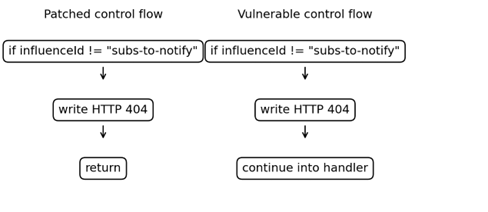
\includegraphics[width=\columnwidth]{figures/fig1.png}
\caption{Simplified control-flow difference between the vulnerable
missing-\texttt{return} path and the corrected path.}
\label{fig:cfg}
\end{figure}

\section{Research Questions}

The case study is organised around four questions, answered directly in
Section~\ref{sec:eval}:

\begin{itemize}
\item \textbf{RQ1.} How much can reachability analysis reduce the scope of
vulnerability triage in the real free5GC UDR source?
\item \textbf{RQ2.} Can reachability-guided analysis identify the functions
relevant to the disclosed CVE family and correctly classify the reachable
findings as CWE-285?
\item \textbf{RQ3.} Can rule-based patch generation produce targeted patches for
the reachable findings while preserving a successful build of the real upstream
free5GC/udr repository?
\item \textbf{RQ4.} What limitations remain after upstream build verification,
particularly regarding complete vulnerability correction and runtime security
validation?
\end{itemize}

\section{Approach}

\subsection{Reachability filtering}

Following OpenAnt's decomposition methodology~\cite{openant}, we parse the target
source with \texttt{tree-sitter}, a real grammar-based parser rather than a regex
or brace-counting heuristic, build a call graph over all top-level function and
method definitions, and perform a breadth-first traversal from a stated list of
entry points: here, the four real free5GC UDR HTTP handler functions that a
service-based-interface client can invoke directly. Any function not reachable
from those entry points is excluded from the priority path, on the premise that
code an external attacker cannot reach through the declared interface does not
need to be triaged with the same urgency as directly exposed code.

This design deliberately separates two questions that are frequently conflated in
automated security analysis. First: is there an external entry point that can
reach a given piece of code? Second: does the reachable code contain a
vulnerability? The first is answered structurally, from the call graph; the
second by the vulnerability heuristics. Separating the stages lets the reduction
be measured on its own, so no credit for the reachability result is attributed to
the security rule.

\begin{figure}[t]
\centering
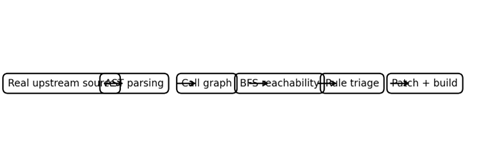
\includegraphics[width=\columnwidth]{figures/fig2.png}
\caption{End-to-end workflow used in the reachability-guided case study.}
\label{fig:workflow}
\end{figure}

\subsection{Call-graph construction}

The parser produces a top-level call graph of functions and methods. The four
UDR HTTP entry points invoked by a service-based-interface client are the roots
of the breadth-first traversal; the reachable subgraph is exactly the set carried
forward to triage. Figure~\ref{fig:callgraph} illustrates the externally
reachable subgraph conceptually.

\begin{figure}[t]
\centering
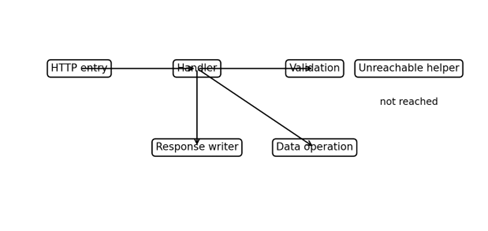
\includegraphics[width=\columnwidth]{figures/fig3.png}
\caption{Conceptual call graph illustrating the externally reachable subgraph
used for triage.}
\label{fig:callgraph}
\end{figure}

\subsection{Triage and patch generation}

Each reachable function is checked against a small library of rule-based
vulnerability patterns. The pattern relevant to this case,
\texttt{find\_missing\_return\_after\_response}, flags a function that writes an
HTTP error response inside a conditional block without a following
\texttt{return} statement in that block --- exactly the control-flow defect
described in Section 2. When the pattern matches, a patch is generated by
inserting a \texttt{return} statement immediately after the flagged response
write. This is a targeted, minimal-diff patch, not a full-function rewrite.

A minimal-diff strategy has two benefits here. First, it makes the intended
correction easy to inspect against the disclosed upstream fix. Second, it
minimises the amount of generated code that must be trusted. The approach is thus
closer to targeted program repair than to code synthesis. The wider project also
contains LLM-based fallback mechanisms; this study deliberately reports only the
deterministic, rule-based path, so that the result cannot be mistaken for a
discovery or for an LLM's generation of this specific fix.

\subsection{Upstream verification}

Prior work verifying a generated patch typically applies it to an isolated copy
of the single affected file and checks that the file alone still compiles. This
does not establish compatibility with the project's actual build: a real Go
module's compilation depends on its full dependency graph, declared in
\texttt{go.mod}/\texttt{go.sum}, and on how the patched function interacts with
the rest of the package. We instead clone the real \texttt{free5gc/udr}
repository at the commit immediately preceding the disclosed fix, confirm the
unmodified repository builds (\texttt{go build ./...}) as a baseline, apply all
generated patches directly to the real
\texttt{internal/sbi/api\_datarepository.go} inside that clone, and rebuild. This
exercises the project's actual dependency graph --- including
\texttt{gin-gonic/gin}, \texttt{go.mongodb.org/mongo-driver}, and free5GC's own
internal packages --- rather than a synthetic stand-in.

\begin{figure}[t]
\centering
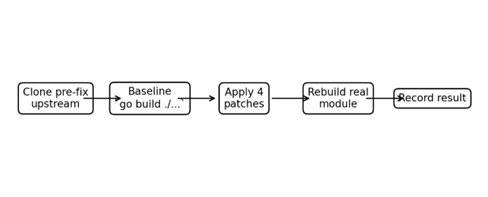
\includegraphics[width=\columnwidth]{figures/fig4.png}
\caption{Upstream verification procedure: baseline build, patch application, and
complete-module rebuild.}
\label{fig:verify}
\end{figure}

\begin{table}[t]
\centering
\caption{Upstream verification stages and observed results.}
\label{tab:verify}
\small
\begin{tabular}{@{}lll@{}}
\toprule
Stage & Purpose & Observed result \\
\midrule
Pre-fix clone & Use real upstream source & Completed \\
Baseline build & Establish unmodified build & \texttt{go build ./...} OK \\
Patch application & Apply the four changes & 4/4 applied \\
Patched build & Check real-dependency fit & \texttt{go build ./...} OK \\
\bottomrule
\end{tabular}
\end{table}

\section{Evaluation}
\label{sec:eval}

\textbf{RQ1: Reachability reduction.} Parsing
\texttt{internal/sbi/api\_datarepository.go} (a real, $\sim$86\,KB source file)
yields 102 top-level functions. Breadth-first traversal from the four real UDR
entry points reaches exactly 4 of them, computed as $(102-4)/102 = 96.1\%$
reduction in the functions a subsequent triage step must consider. This headline
measurement is taken directly from the real source file, not a synthetic
benchmark (Figure~\ref{fig:reduction}).

\begin{figure}[t]
\centering
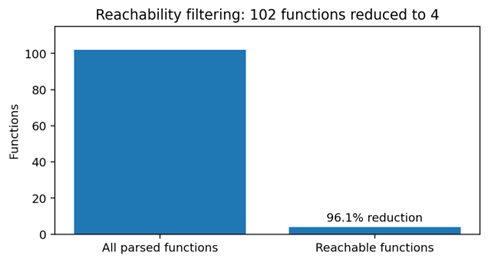
\includegraphics[width=\columnwidth]{figures/fig5.png}
\caption{Measured reduction in the number of functions requiring subsequent
triage.}
\label{fig:reduction}
\end{figure}

\textbf{RQ2: Triage and classification.} The missing-\texttt{return} rule matches
all four reachable functions, and each is classified as CWE-285, matching the
disclosed class for this CVE family. Table~\ref{tab:handlers} lists the four
handlers; all share the prefix
\texttt{HandleApplicationDataInfluenceDataSubsToNotify}, omitted for space. The
agreement among the reachability result, the rule-based classification, and the
disclosed upstream vulnerability gives focused validation of the pipeline for
this case.

\begin{table}[t]
\centering
\caption{Reachable UDR handlers and generated patch outcomes.}
\label{tab:handlers}
\small
\begin{tabular}{@{}lccc@{}}
\toprule
Handler suffix & HTTP verb & Missing \texttt{return}s & Patched \\
\midrule
\texttt{SubscriptionIdPut} & PUT & 1 & Full \\
\texttt{SubscriptionIdGet} & GET & 1 & Full \\
\texttt{SubscriptionIdDelete} & DELETE & 1 & Full \\
\texttt{Get} (list) & GET & 2 & Partial (1/2) \\
\bottomrule
\end{tabular}
\end{table}

\textbf{RQ3: Patch generation and upstream verification.} A patch is generated
for all four flagged functions. The unmodified clone builds cleanly as a
baseline. With all four generated patches applied directly to the real,
live-cloned repository, \texttt{go build ./...} again succeeds against the
project's actual dependency graph (Table~\ref{tab:verify}). As far as we are
aware, this is the first time a patch produced by this reachability pipeline has
been verified against a real upstream module's full dependency graph rather than
an isolated single-file copy (Figure~\ref{fig:patchout}).

\begin{figure}[t]
\centering
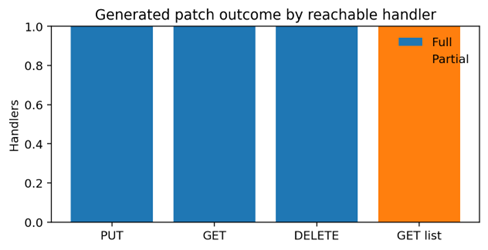
\includegraphics[width=\columnwidth]{figures/fig6.png}
\caption{Patch-generation outcomes across the four reachable handlers.}
\label{fig:patchout}
\end{figure}

\textbf{RQ4: Remaining limitations.} One of the four handlers, the list-GET
handler, requires \emph{two} separate \texttt{return} insertions in the real
disclosed fix (two independent conditional blocks in the same function body),
while the rule-based patcher returns only the first match per function. That
handler is therefore only partially corrected: the build still succeeds (a
partial fix does not break compilation), but the vulnerability is not fully
closed for that one handler. This is a genuine, measured limitation of a
single-finding-per-pattern-match design, not a flaw discovered after
publication. A clean build also remains a compile-time observation only: it shows
the generated changes are accepted by the Go compiler and introduce no
dependency or type errors, but it does not by itself prove the endpoint is safe
at runtime in every deployment. Section~\ref{sec:disc} develops both limits.

\section{Analysis of the Security Mechanism}

This vulnerability family illustrates why compilation alone is insufficient and
why reachability and control-flow reasoning add value. The validation branch of
each handler correctly refuses an invalid influence identifier and emits an HTTP
error, but that is only half of the required behaviour: the handler must also
terminate so that subsequent state-changing actions do not run. The fault is a
mismatch between the intended security policy and the realised control-flow
graph. In the pipeline, static parsing exposes the function's structure, the
rule detects the missing termination, and patch generation supplies it ---
each stage contributing a distinct, inspectable piece of evidence
(Table~\ref{tab:components}).

\begin{table}[t]
\centering
\caption{Separation of analysis components and evidence type.}
\label{tab:components}
\small
\begin{tabular}{@{}lll@{}}
\toprule
Component & Role in this case & Evidence type \\
\midrule
Tree-sitter & Parse Go source & Structural \\
Call graph + BFS & Identify reachable functions & Measured \\
Rule heuristic & Detect missing \texttt{return} & Rule match \\
Patch generator & Insert targeted \texttt{return} & Generated diff \\
Go compiler & Check full-module fit & Build evidence \\
\bottomrule
\end{tabular}
\end{table}

\textbf{Relationship to LLM-assisted security.} This case study is deliberately
deterministic --- reachability, a rule, and a compiler --- so that its evidence
reproduces independently of model variance. That is a scoping choice, not a claim
that language models have no role: an LLM can usefully explain code, propose
hypotheses, generate patch alternatives, or perform adversarial review, while
structural reachability and compiler checks act as deterministic evidence gates
around it. The result reported here comes from the rule-based path and is not a
benchmark for any live model.

\section{Discussion and Limitations}
\label{sec:disc}

A clean build after patching establishes that a generated patch is syntactically
valid and compatible with the real project's dependency graph. It does not
establish that the patch is correct at runtime. Confirming that the vulnerability
is actually closed would require running the real free5GC UDR service and sending
it a live HTTP request, which in turn requires the rest of the deployment this
network function depends on: a MongoDB backend for its data store and
registration with the free5GC NRF for service discovery. Standing up that
deployment was outside the scope of this case study and is the most direct next
step for this work (Figure~\ref{fig:boundary}).

\begin{figure}[t]
\centering
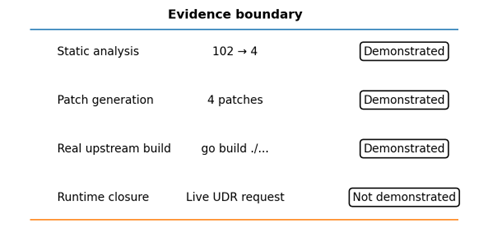
\includegraphics[width=\columnwidth]{figures/fig7.png}
\caption{Evidence boundary of the experiment: what is demonstrated and what
remains unverified.}
\label{fig:boundary}
\end{figure}

\textbf{Scope of generalisation.} This is a single-file, single-family case
study. It evaluates one real free5GC component, one disclosed vulnerability
family (two CVEs), and one missing-\texttt{return} control-flow pattern in Go.
The 96.1\% reduction observed for this file and this set of HTTP entry points
illustrates the effect of reachability filtering, but the figure will vary with
project, language, architecture, and vulnerability type. Likewise, a patch that
compiles is compatible with the tested upstream dependency graph, not necessarily
correct in all cases. Broader conclusions would require several repositories,
vulnerability classes, languages, and runtime security tests under reproducible
conditions.

\textbf{Partial-patch limitation.} The most concrete limitation is the list-GET
handler's two-insertion fix: the current rule captures only the first match per
function, and compilation does not reveal the incompleteness. The natural
improvement is to have the patch interface emit all safe matches within a
function, then re-run the upstream build and, ideally, a runtime regression test.

\textbf{Threats to validity.} Internal validity is supported by using real
upstream source, a fixed set of entry points, a real grammar-based parser, and a
full-module build. Reachability is a property of the static call graph and does
not by itself prove a function is reachable in every runtime configuration.
External validity is limited by the single case. The study is reproducible ---
the source is vendored, the commit hashes recorded, and the verification commands
captured --- but results may be influenced by environmental differences such as
Go toolchain version, module availability, and network access.

\section{Related Work}

Our reachability filtering directly follows OpenAnt~\cite{openant}, which combines
reachability-based code decomposition with LLM-driven adversarial verification
and sandboxed dynamic testing to discover previously unknown vulnerabilities
across projects including OpenSSL, WordPress, and Flowise, reporting up to 97\%
reduction in analysis scope. We apply the same decomposition step to a single,
real, disclosed CVE family rather than searching for unknown bugs, and add a
verification step OpenAnt's own evaluation does not report: confirming a
generated patch against a live clone of the real upstream repository.

DARPA's AI Cyber Challenge (AIxCC) produced seven open-sourced cyber-reasoning
systems combining fuzzing, static analysis, and LLM agents for autonomous
vulnerability discovery and patching~\cite{aixcc}. FuzzingBrain, a fourth-place
AIxCC finalist, autonomously discovered 28 vulnerabilities (including six
zero-days) in real C and Java projects and patched 14, using LLMs as semantic
navigators over reachability-partitioned code before dynamic
verification~\cite{fuzzingbrain}; its \emph{analyse $\rightarrow$ direction
$\rightarrow$ verify} shape mirrors this study's reachability $\rightarrow$
triage $\rightarrow$ build-verification pipeline, independently arrived at by a
funded finalist team. OSS-CRS extends this line of work by porting AIxCC-era
systems to real OSS-Fuzz projects under resource budgets~\cite{osscrs}. Our work
is narrower than all of these: we do not attempt discovery of unknown
vulnerabilities, only reachability-filtered triage and patching of already
disclosed ones. It shares their emphasis on evaluating against real, not
synthetic, targets (Table~\ref{tab:related}).

\begin{table}[t]
\centering
\caption{Positioning against related security-automation work.}
\label{tab:related}
\small
\begin{tabular}{@{}lll@{}}
\toprule
Work & Primary focus & Relation to this study \\
\midrule
OpenAnt~\cite{openant} & Reachability + LLM analysis & Methodological basis \\
AIxCC~\cite{aixcc} & Autonomous cyber reasoning & Broader context \\
FuzzingBrain~\cite{fuzzingbrain} & LLM-guided discovery+patch & Same pipeline shape \\
OSS-CRS~\cite{osscrs} & Real OSS workloads & Real-target motivation \\
This work & Reachability + patch + build & Focused free5GC case \\
\bottomrule
\end{tabular}
\end{table}

\textbf{Difference from synthetic validation.} This study should not be read as a
replacement for dynamic testing. Static reachability narrows the code to inspect,
and compiler verification catches integration errors, but neither replaces a real
security test. The strongest future evaluation would connect the tested static
pipeline to a real free5GC deployment and replay the request that demonstrated
the vulnerability before the patch against the patched endpoint.

\section{Reproducibility}

The \texttt{src/reachability/} module and its documentation are hosted in the
project repository for the free5GC case~\cite{fyprepo}. Both vulnerable and
patched versions of the source are retained as case-study inputs, with the
pre-fix and fix commit hashes recorded. The static procedure runs from the
vendored case-study source; upstream verification clones the real module and runs
the full Go build. Table~\ref{tab:repro} lists the minimum record needed to
reproduce each reported number.

\begin{table}[t]
\centering
\caption{Minimum reproducibility record.}
\label{tab:repro}
\small
\begin{tabular}{@{}lll@{}}
\toprule
Artifact & Purpose & Recorded value \\
\midrule
Source commit & Fix provenance & Git hash \\
Toolchain & Reproduce parse/build & Versions \\
Entry points & Reachability boundary & 4 handler names \\
Analysis result & Filtering measure & 102 / 4 / 96.1\% \\
Patch result & Generated edits & 4 generated; 1 partial \\
Build result & Integration check & Baseline OK; patched OK \\
\bottomrule
\end{tabular}
\end{table}

\section{Future Work}

First, runtime verification against a real free5GC UDR service: deploy the UDR
with its MongoDB backend and NRF registration, replay the vulnerable request
against the pre-fix revision, apply the generated patch, and replay again. A
demonstrated negative that also preserves legitimate subscription behaviour would
be far stronger evidence than compilation alone. Second, extend the patch
generator to emit multiple edits per function: the present restriction to the
first matching conditional block is exactly what leaves the list-GET handler
partially corrected, and emitting all safe matches, then checking for conflicts
and rebuilding, is the direct fix. Third, evaluate additional free5GC components
and vulnerability classes to test whether the reduction and patch-success
observations hold beyond this one file and family.

\section{Conclusion}

We presented a focused case study on a publicly disclosed vulnerability family in
free5GC, showing that reachability-filtered static analysis and rule-based patch
generation can be applied to a real vulnerability in an actual project's upstream
repository. The analysis narrowed 102 real functions to the 4 reachable handlers
that matter --- a 96.1\% reduction --- classified all four as CWE-285 matching
the disclosed class, and produced patches that, applied to the real upstream
module, preserve a clean \texttt{go build ./...} against the project's actual
dependency graph. We report this alongside its real limits: one handler is only
partially corrected because the rule emits one match per function, and a
successful build is not runtime confirmation. The contribution is not a claim of
autonomous or complete remediation; it is a reproducible, real-target
demonstration that reachability filtering focuses analysis and that upstream
build verification provides more integration evidence than single-file
compilation. The method extends naturally toward runtime security verification
and a larger corpus of network-function software.

\begin{thebibliography}{9}

\bibitem{openant}
Nahum Korda and Gadi Evron. 2026. OpenAnt: LLM-Powered Vulnerability Discovery
Through Code Decomposition, Adversarial Verification, and Dynamic Testing.
\textit{arXiv preprint arXiv:2606.19149} (2026).
\url{https://arxiv.org/abs/2606.19149}

\bibitem{free5gc}
free5GC Project. \url{https://free5gc.org/}.

\bibitem{aixcc}
DARPA. 2025. AI Cyber Challenge marks pivotal inflection point for cyber defense.
(August 2025). \url{https://www.darpa.mil/news/2025/aixcc-results}

\bibitem{osscrs}
Andrew Chin, Dongkwan Kim, Yu-Fu Fu, Fabian Fleischer, Youngjoon Kim, HyungSeok
Han, Cen Zhang, Brian Junekyu Lee, Hanqing Zhao, and Taesoo Kim. 2026. OSS-CRS:
Liberating AIxCC Cyber Reasoning Systems for Real-World Open-Source Security.
\textit{arXiv preprint arXiv:2603.08566} (2026).
\url{https://arxiv.org/abs/2603.08566}

\bibitem{fuzzingbrain}
Ze Sheng, Qingxiao Xu, Jianwei Huang, Matthew Woodcock, Heqing Huang, Alastair F.
Donaldson, Guofei Gu, and Jeff Huang. 2025. All You Need Is A Fuzzing Brain: An
LLM-Powered System for Automated Vulnerability Detection and Patching.
\textit{arXiv preprint arXiv:2509.07225} (2025).
\url{https://arxiv.org/abs/2509.07225}

\bibitem{kuznetsov}
Alexandr Kuznetsov, Yehor Yeromin, Oleksiy Shapoval, Kyryl Chernov, Maryna
Popova, and Konstantin Serdukov. 2019. Automated Software Vulnerability Testing
Using Deep Learning Methods. In \textit{2019 IEEE 2nd Ukraine Conference on
Electrical and Computer Engineering (UKRCON)}. IEEE, 837--841.
\url{https://doi.org/10.1109/UKRCON.2019.8879997}

\bibitem{almazyad}
Ibrahim Almazyad, Safwan Elmadani, and Salim Hariri. 2024. A 5G and Beyond
Testbed for Cybersecurity Research and Education. In \textit{2024 IEEE/ACS 21st
International Conference on Computer Systems and Applications (AICCSA)}. IEEE,
1--6.

\bibitem{udrfix}
free5GC/udr. CVE-2026-40248 / CVE-2026-40246 fix, upstream commit
\texttt{86686276a7e226183ee786e3dd6714ec56c78fda}, 2026.

\bibitem{fyprepo}
Jothilingam Dheeraj. 2026. Final-Year-Project (\texttt{src/reachability/}).
GitHub repository. \url{https://github.com/J-Dheeraj/Final-Year-Project}

\end{thebibliography}

\end{document}
